\clearpage
\section{Webserver (AW)}
\label{section_webserver}
Der Webserver nimmt Anfragen des Clients über HTTP entgegen. Er liefert zum einen die 
Internetseite an den Client aus, über die der Benutzer mit der Anwendung interagiert und 
kommuniziert zum anderen mit dem Datenserver.

Der typische Ablauf der Kommunikation zwischen Webclient und Webserver ist in der 
folgenden Abbildung \ref{fig_webserver_webclient} dargestellt:

\begin{figure}[h]
	\centering
	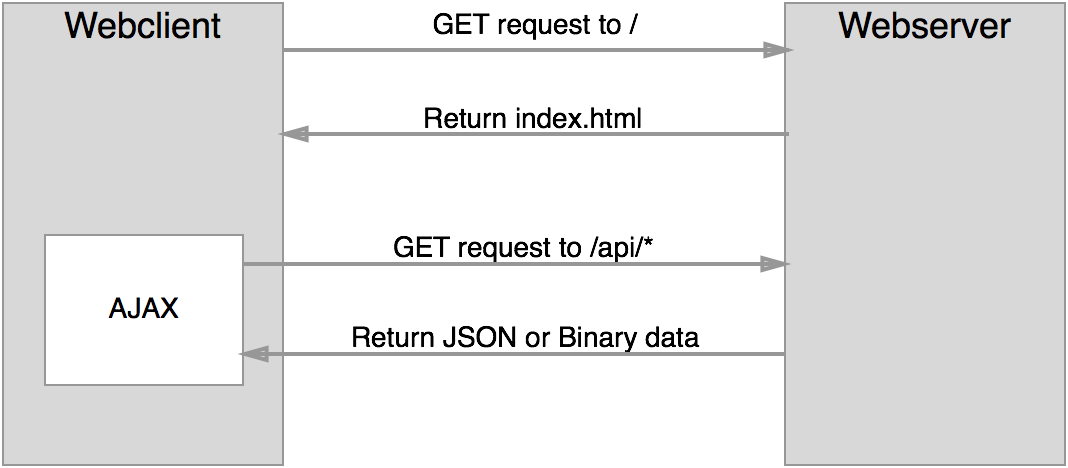
\includegraphics[width=\textwidth]{bilder/abbildung_webserver_webclient}
	\caption{Kommunikation zwischen Webclient und Webserver}
	\label{fig_webserver_webclient}
\end{figure}

Die Abbildung zeigt, wie der Webserver eine Anfrage an 
den Webserver stellt und der mit der Rückgabe der Datei \textit{index.html} antwortet. Da es sich um eine Single-Page-Anwendung handelt, liefert der Webserver nur dieses eine Seite / Page aus.

In der Abbildung \ref{fig_webserver_webclient} ist weiter vereinfacht dargestellt, wie die weitere Kommunikation zwischen Webclient und Webserver über die im Webclient integrierte AJAX\footnote{AJAX (Asynchronous JavaScript and XML): Konzept zur asynchronen Datenübertragung}-Engine ausgeführt wird.
\clearpage
\subsection{Schnittstellen}
Der Webserver hält die in der folgende Tabelle \ref{tab_api_routes} dargestellten Schnittstelle bereit, an die der Webclient 
Anfragen richten kann:
\begin{table}[h]
	\begin{center}
		\begin{tabularx}{\textwidth}{|c|l|X|}
			\hline
			\textbf{Methode} & \textbf{Pfad} & \textbf{Funktion}\\
			\hline
			GET & / & ruft die Datei index.html auf und bewirkt den Start der Anwendung \\
			\hline
			GET & /api/sessions/:id & ruft die Session mit gegebenen ID auf \\
			\hline
			GET & /api/thumbnails/:id & ruft ein Thumbnail des Bildes mit gegebenen ID ab \\
			\hline
			GET & /api/images/:id & ruft ein Bild mit gegebenen ID ab \\
			\hline
		\end{tabularx}
		\caption{Die zu realisierende Schnittstelle}
		\label{tab_api_routes}
	\end{center}
\end{table}

Die in Tabelle angegeben Endpunkte werden wie folgt verwendet:

Der Pfad "/"{} wird durch den Browser des Clients über die Eingabe des Domainnamens aufgerufen.

Der Pfad "/api/sessions/:id"{} wird über einen AJAX-Request aufgerufen, wenn auf der Startseite eine Session-ID 
eingeben wird und der Benutzer den Knopf  "Senden" drückt.

Die Pfade "/api/thumbnails/:id"{} und "/api/images/:id"{} werden in der Datei \textit{index.html} als Attribute des Tags \textit{\textless img\textgreater} verwendet.

\subsection{Realisierung}
Der Webserver ist in JavaScript auf der Node.js-Plattform implementiert. Zur vereinfachten Installation und bequemeren Handhabung von Anfragen an den Server wird das Framework \textit{Express.js} verwendet. 
\clearpage
Die Darstellung der Ordnerstruktur enthält folgende Abbildung \ref{fig_struktur_webserver}:
\begin{figure}[h]
	\centering
	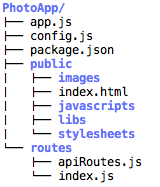
\includegraphics[width=4cm]{bilder/ordnerstruktur_photoapp}
	\caption{Ordnerstruktur des Webservers}
	\label{fig_struktur_webserver}
\end{figure}

Die Datei \textit{package.json} enthält die Konfiguration einer Node.js-Anwendung und 
definiert unter anderem Abhängigkeiten zu Paketen.

Die Datei \textit{config.js} enthält die URL und Ports der beteiligten Server.

In der Datei \textit{app.js} sind die Befehle zur Erzeugung des Web-Servers enthalten. Weiter werden in dieser Datei die übrigen Dateien und die Routen importiert. In Listing \ref{list_server} ist die Datei auszugsweise vorgestellt.

\begin{figure}[h]
\begin{lstlisting}[caption={Auszug aus app.js}, label=list_server]
var express	= require("express"); // import express.js module
var app		= express(); // initialize app / server
var indexRoutes = require("'./routes/index"); // import routes
var apiRoutes = require("./routes/apiRoutes"); // import more routes

app.use("/", routes); // use routes for requests to server
app.listen(60127); // start server listening on port 60127
\end{lstlisting}
\end{figure}

Das Listing zeigt, wie zunächst die verwendeten Module mit \textit{require} importiert werden und die Anwendung anschließend Anwendung initialisiert wird. Im Anschluss werden die importierten Routen in die Anwendung integriert und zum Schluss der Server gestartet. Der Server hört auf Anfragen an den definierten Port.

Die einzelnen Endpunkte der Schnittstelle (Routen) sind wie in Listing \ref{list_api} abgebildet implementiert:

\begin{figure}
\begin{lstlisting}[caption={Auszug aus den Dateien routes/index.js und routes/apiRoutes.js}, label=list_api]
/* GET home page. */
router.get("/", function(req, res, next) {
    res.sendFile('index.html');
});

/* GET requests to /api/sessions/:id, /api/thumbnails/:id, /api/images/:id */
router.get("/sessions/:id", function(req, res, next) {
    var sessionId = req.params.id;
    // create options object for the following request
	var options = {
		host: serverData.host,
		port: serverData.port,
		path: "/api/sessions/" + sessionId,
		method: "GET",
		accept: "application/json"
	};

	// create and send request
	http.request(options, function(response) {
	// check response for error
	    if (response.statusCode == "404") {
	        return res.status(404).send();
		}
		// in case of images pipe incoming stream to outgoing stream
		// response.pipe(res);
		
		var resData = "";
		// react to the server's response...
		response.on("data", function(data) {
		// ... by passing the responded data to variable resData...
		    resData += data;
		});
		
		// ...and returning it to the client in the end
		response.on("end", function() {
		    // ...as JSON if dealing with session data...
		    res.json(JSON.parse(resData));
		    // ...or as binary data in case of images
		    // res.set("Content-Type", contentType);
		    // res.end(resData, "binary");
		});
	}).end();
});
\end{lstlisting}
\end{figure}

Die erste Route in den Zeilen 2-4 reagiert auf die Anfrage an den Pfad "/".
Sie sendet daraufhin die HTML-Datei an den Client zurück.

Die zweite Route in den Zeilen 7 bis 40 ist verantwortlich für Anfragen an den Pfad 
"/api/sessions/:id", die Funktionsweise ist jedoch identisch zur Anfragen 
an "/api/images/:id"{} und "/api/thumbnails/:id".

Wenn eine Anfrage an diese Pfade eingeht, wird eine entsprechende HTTP-Anfrage 
an den Datenserver gerichtet und die zurückerhaltene Antwort an den Webclient 
weitergeleitet.

Zunächst wird aus den Request-Parametern die ID ausgelesen (Zeile 8). Anschließend 
wird ein Objekt erzeugt, das die Art der ausgehenden HTTP steuert (Zeilen 10-16).
Der HTTP Request wird mit den gegebenen Optionen an den Datenserver gesandt (Zeile 19 bis 42).
Die zurückkommende Antwort wird verarbeitet und an den Webclient weitergeleitet (Zeilen 21 bis 40).

Die Anwendung enthält im Übrigen den Ordner \textit{public}, der die Dateien des Webclients 
enthält (vgl. Abschnitt \ref{section_webclient}).


